\documentclass{beamer}
\mode<presentation> {
	\usetheme{Madrid}
}
\usepackage[slovak]{babel}
\usepackage[utf8]{inputenc}
\usepackage{amsmath}
\usepackage{graphicx}
\usepackage{booktabs}
\usepackage{color}

\usepackage{hyperref}
\newcommand\crule[1][black]{\textcolor{#1}{\rule{0.25cm}{0.25cm}}}
\DeclareUnicodeCharacter{00A0}{~}

%----------------------------------------------------------------------------------------
%	TITLE PAGE
%----------------------------------------------------------------------------------------

\title[]{Jet-like correlations with neutral pion triggers in pp and central Pb-Pb collisions at 2.76 TeV} 

\author{Lucia Anna Husová} 
\institute[UPJŠ] 
{
	Prírodovedecká fakulta\\
	Univerzita Pavla Jozefa Šafárika \\ 
	
	
}
\date{5.12.2016} 

\begin{document}
	
	\begin{frame}
		\titlepage
	\end{frame}
	
	\begin{frame}
	\frametitle{Obsah}
		\tableofcontents 
	\end{frame}
	
	\section{Úvod}
	\begin{frame}
		\frametitle{Motivácia}
		\begin{itemize}
			\item Zrážky relativistických ťažkých iónov $\rightarrow$ vznik QGP 
			\item Dôkaz existencie QGP - jet quenching
			\item Pozorovaná na RHIC a LHC - merania produkcie hadrónov a jetov pri vysokých $p_T$, dvojhadrónových uhlových korelácií, nerovnováhy energie 2 jetov ...
			\item Pomocou korelácií - štúdium vzájomného pôsobenia mäkkých a tvrdých procesov
			\item Na RHICu - "double-shoulder" štruktúra na away side píku $\rightarrow$ vysvetlené Čerenkovovým gluónovým žiarením, odklonením jetu médiom,... $\rightarrow$ 
			korelácie sú ovplyvnené vyššími rádmi harmonického toku $\rightarrow$ potreba vziať do úvahy anizotropický tok pozadia vyšších rádov
		\end{itemize}
	\end{frame}
	
	\begin{frame}
		\frametitle{Metóda}
		\begin{itemize}
			\item Štúdium dvojčasticových korelácií:
			\begin{itemize}
				\item trigger: $\pi^{0}$ s $8<p_T^{trigg}<16GeV/c$
				\item assoc. častice: nabité hadróny s $0.5<p_T^{assoc}<10GeV/c$
				\item $\Delta\varphi$ v strednej rapidite 
				\item pp a centrálne Pb-Pb zrážky pri $\sqrt{s_{NN}}=2.76TeV$
				\item $\pi^{0}$ rekoštruované cez kanál $\pi^{0} \rightarrow \gamma \gamma$ použitím shower shape metódy a invariatnej hmotnosti (EMCal)
				\item Dráhy hadrónov rekonštruované v TPC a ITS
				\item Počítané: výťažky pre $\lvert\Delta \varphi\rvert < 0.7$ a $\lvert\Delta \varphi - \pi\rvert < 1.1$ a $I_{AA}$
				\item Výsledky porovnané s modelmi energetických strát partónov (generátory JEWEL a AMPT), poruchovou QCD a výsledkami z RHIC
			\end{itemize}
		\end{itemize}
	\end{frame}
	
	\section{Detektory a datasety}
	\begin{frame}
		\frametitle{Detektory a datasety}
		\begin{itemize}	
			\item Dáta z roku 2011 pri $\sqrt{s_{NN}}=2.76TeV$
			\item Selekcie:
			\begin{itemize}	
				\item pp zrážky - EMCal level0 trigger vyžadoval jedinú spŕšku s $E>3GeV$
				\item Pb-Pb - online trigger vyberal iba centrálne zrážky s efektivitou 100\% pre 0-8\% a 80\% pre 8-10\% centralitu
				\item Rekonštruovaný vertex $\lvert z_{vrx}\rvert<10cm$
			\end{itemize}	
			\item Po selekciách analyzovaných 440 tisíc prípadov pre pp a 5.2 miliónov prípadov pre Pb-Pb
		\end{itemize}

	\end{frame}
	
	
	\begin{frame}
		\frametitle{Detektory a datasety}
		\begin{itemize}
			\item $\pi^{0}$ v $\lvert\eta\rvert<0.7$ identifikované v EMCal metódou "cluster splitting"
			\item Clustre z neutrálnych častíc sú identifikované, ak vzdialenosť medzi extrapolovanou polohou tracku a clustrom spĺňa $\Delta \eta >0.025$ a 
			$\Delta \varphi >0.03$ pre pp a $\Delta \eta >0.03$ a $\Delta \varphi >0.035$ pre Pb-Pb
			\item Nabité hadróny selektované pomocou hybridného prístupu a musia spĺňať $DCA < 2.4 cm$ v rovine kolmej na zrážku a $DCA < 3 cm$ v smere zrážky
			\item Tracky akceptované ak $\lvert\eta\rvert<0.8$ a $p_T>0.5 GeV$
			\item Korekcie vzhľadom na detektor pomocou MC simulácií - PYTHIA6, HIJING a GEANT3
		\end{itemize}
	\end{frame}
	
	\section{Analýza}
	\begin{frame}
		\frametitle{Analýza}
		\begin{itemize}
			\item[] \begin{equation}
			         \centering M_{\pi^0}=\sqrt{2E_1E_2(1-cos\thetha_{12})} 
			        \end{equation}

			\item Čím vyššia energia $\pi^{0}$ $\rightarrow$ spájanie clustrov v EMCal, tie sú identifikované podľa tvaru spŕšky parametrom $\lambda_{0}$
			\item Na rozlíšenie spojených clustrov a jednofotónového prípadu $\rightarrow$ $\lambda_{0}>0.3$
			\item[] \centering 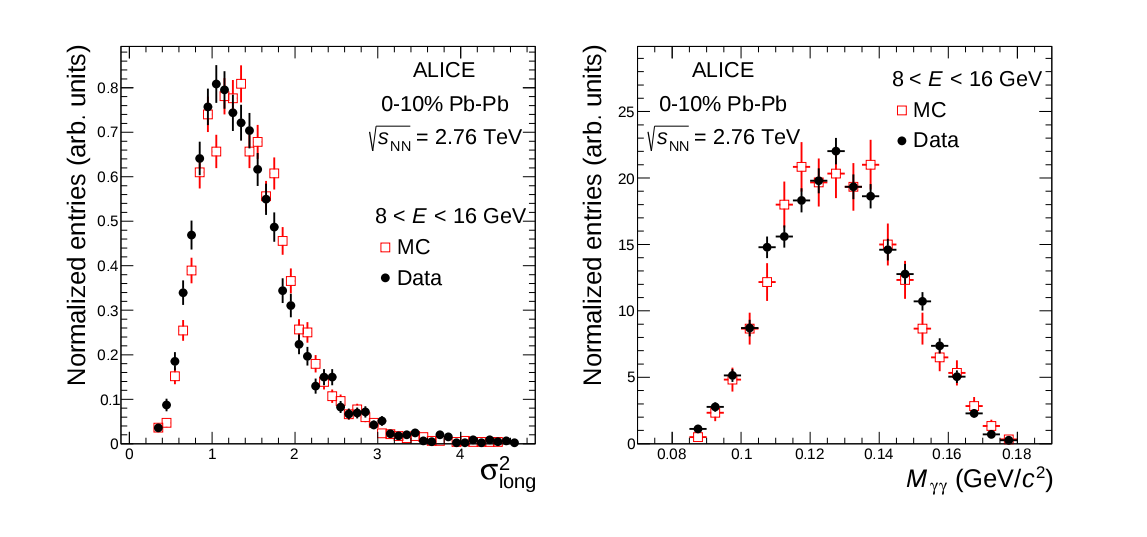
\includegraphics[scale=0.18]{./Obrazky/lambda0.png}
		\end{itemize}
	\end{frame}
	
	\begin{frame}
		\frametitle{Analýza}
		\begin{itemize}	
		 \item Výťažok: 
		 \item[]  \begin{equation} \centering 
		          Y(\Delta\varphi,\Delta\eta)=\frac{1}{N_{trig}}\frac{d^2N_{assoc}}{d\Delta\varphi\Delta\eta}
		          \end{equation}
		 \item akceptancia triggra je $\lvert\eta\rvert<0.7$ a assoc. častíc $\lvert\eta\rvert<0.8$ $\rightarrow$ korigovaný výťažok:
		 \item[]  \begin{equation} \centering
		          \frac{1}{N_{trig}}\frac{d^2N_{assoc}}{d\Delta\varphi\Delta\eta}=\frac{S(\Delta\eta,\Delta\varphi)}{M(\Delta\eta,\Delta\varphi)}
		          \end{equation}
		 \item Konečné výsledky sú integrované cez $\eta$ pre $8<p_T^{trigg}<16GeV/c$ a $0.5<p_T^{assoc}<10GeV/c$ ako 1D rozdelenie:
		 \item[]  \begin{equation} \centering
		          C(\Delta\varphi)=\frac{1}{N_{trig}}\frac{dN_{assoc}}{d\Delta\varphi}
		          \end{equation}
		\end{itemize}

	\end{frame}
	
	\begin{frame}
		\frametitle{Analýza}
		\begin{itemize}
			\item \footnotesize {Pre získanie čistého výťažku $\rightarrow$ odčítanie pozadia:}
			\item[]\footnotesize  {\begin{equation} \centering
			         J(\Delta\varphi)=C(\Delta\varphi) - B(\Delta\varphi)
			         \end{equation}}
			\item \footnotesize {Pre pp zrážky - konštantné pozadie $B_0$, pre Pb-Pb pozadie ovplyvnené anizotropickým tokom:}
			\item[]  \footnotesize {\begin{equation}\centering
			         B(\Delta\varphi)=B_0 (1+2\displaystyle\sum_{n}V_n cos(n\Delta\varphi))
			         \end{equation}}
			\item \footnotesize {$V_n$ z predchádzajúcich meraní, $B_0$ priemer z troch hodnôt:}
			\begin{itemize}	
				\item \scriptsize {fit $1<\abs{\Delta\varphi}<\frac{\pi}{2}$}
				\item \scriptsize {8 najmenších hodnôt v celom intervale $\Delta\varphi$}
				\item \scriptsize {minimum v $1<\lvert\Delta\varphi\rvert<\frac{\pi}{2}$}
			\end{itemize}	
			\item \footnotesize {Po odčítaní pozadia $\rightarrow$ výťažok získaný integrovaním na intervaloch $\lvert\Delta \varphi\rvert < 0.7$ a $\lvert\Delta \varphi - \pi\rvert < 1.1$}
			\item \footnotesize {Modifikácia výťažku: \begin{equation}
						   I_{AA}=\int_X J_{AA} (\Delta\varphi) d\Delta\varphi / \int_X J_{pp} (\Delta\varphi) d\Delta\varphi
						   \end{equation}}
			
		\end{itemize}
	\end{frame}
	
	\section{Chyby merania}
	\begin{frame}
		\frametitle{Chyby merania}
		\centering 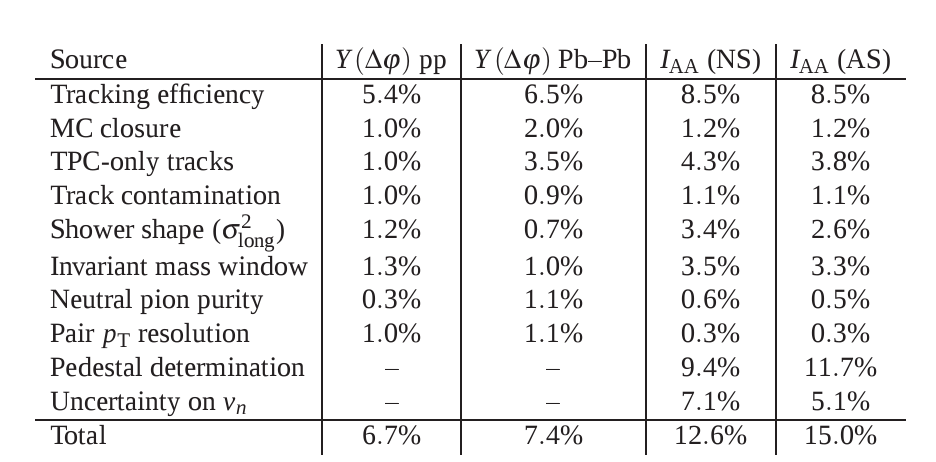
\includegraphics[scale=0.35]{./Obrazky/nepresnosti.png}
	\end{frame}
	
	\section{Výsledky}
	\begin{frame}
		\frametitle{Výsledky - korelácie pp}
		\centering 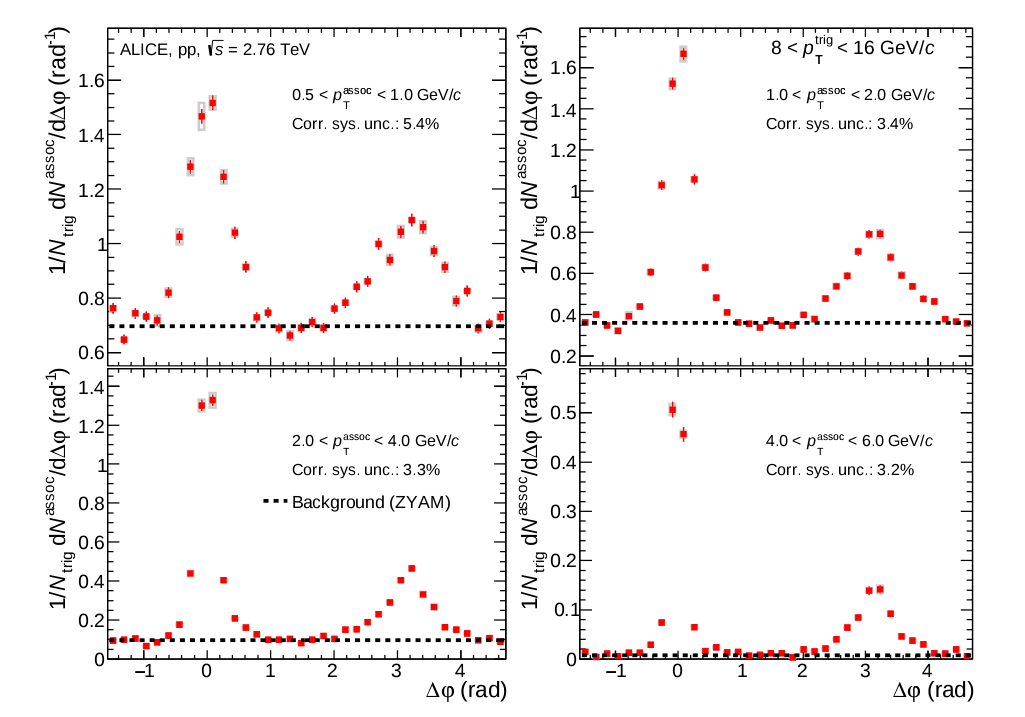
\includegraphics[scale=0.3]{./Obrazky/korelacie.png}
	\end{frame}
	
	\begin{frame}
		\frametitle{Výsledky - korelácie pp}
		\centering 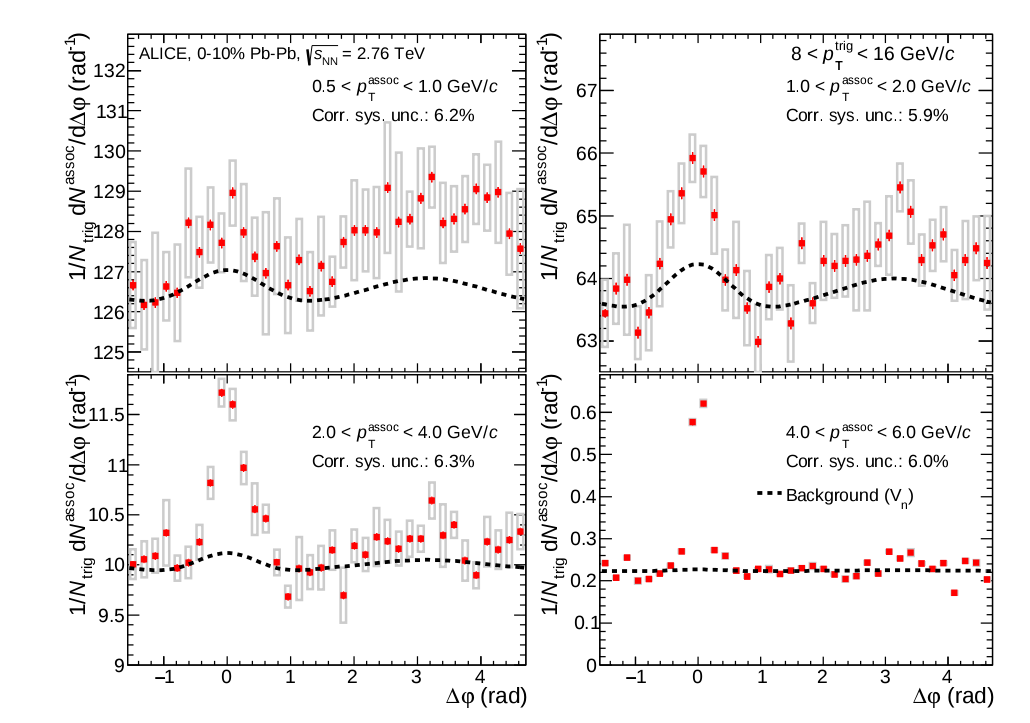
\includegraphics[scale=0.3]{./Obrazky/pozadie.png}
	\end{frame}
	
	\begin{frame}
		\frametitle{Výsledky}
		\centering 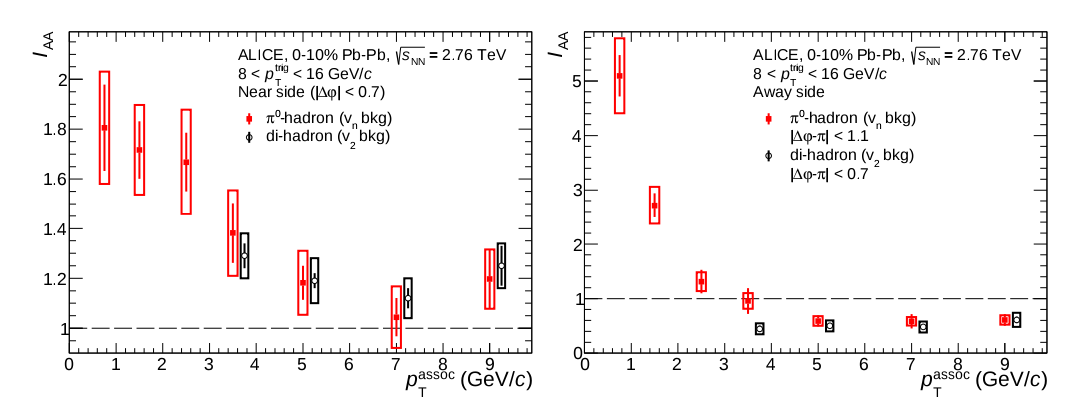
\includegraphics[scale=0.3]{./Obrazky/Iaa.png}
	\end{frame}
	
	\begin{frame}
		\frametitle{Výsledky}
		\centering 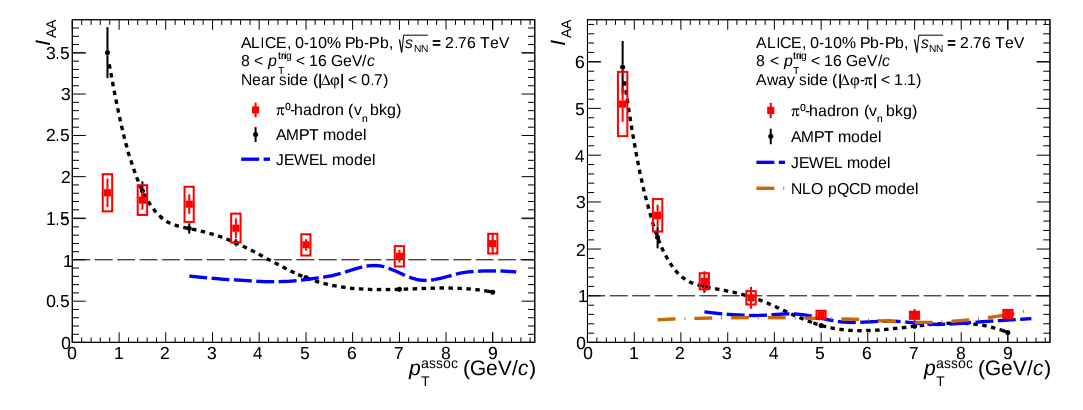
\includegraphics[scale=0.3]{./Obrazky/MC.png}
	\end{frame}
	
	\section{Záver}
	\begin{frame}
		\frametitle{Záver}
		\begin{itemize}
		 \item Pozorované potlačenie $I_{AA}\approx0.6$ na away side pre $p_T^{assoc}>3GeV/c$ 
		 \item Pozorované zvýšenie $I_{AA}\approx5.2$ na away side pre najnižšie $p_T^{assoc}$ 
		 \item Pozorované zvýšenie $1.2<I_{AA}<1.8$ na near side pre najnižšie $p_T^{assoc}$ 
		 \item Všetky modely kvantitatívne popisujú potlačenie pre vysoké $p_T^{assoc}$  na away side
		 \item AMPT popisuje zvýšenie pre nízke $p_T^{assoc}$ na near aj away side
		\end{itemize}

	\end{frame}
	
\end{document}